\chapter{Krunimír: želví grafika}

\begin{quotation}

Želvák Krunimír je velký myslitel. Zjistil, ze když si za krunýř přiváže trochu
křídy, kreslí za sebou při svém plazení cestičku. I pojal plán nakreslit svoji
podobiznu, samozřejmě včetně přesných detailů krunýře. Hned se dal pln nadšení
do díla a práce mu šla pěkně od ... tlapy.

\uv{Co to děláš, dědečku,} zeptal se jednou Krunimíra jeho vnuk Krunoslav.
\uv{Krešlím tady švou poďobižnu,} odpověděl Krunimír. \uv{Žačal jsem š ní, když
tvůj tatík ještě nebyl na švětě, a ještě nemám ani krunýř,} dodal smutně. \uv{To
už ji aši dokrešlit neštihnu...}  Vnuk Krunoslav, znalec moderní techniky, mu
však poradil: \uv{Tak si nech napsat program, který ji nakreslí za Tebe.}
Protože se ale s tlapami a zobákem moc dobře neprogramuje, najali si želváci
vás.
\end{quotation}

Takto začíná zadání finální úlohy Soutěže v programování z roku
2010 \cite{krunimir-task}. Popisuje jednoduchý procedurální jazyk na generování
želví grafiky, inspirovaný jazykem Logo, a úkolem je vytvořit interpret tohoto
jazyka, jehož vstupem je text programu a výstupem vykreslený obrázek. 

\begin{figure}
  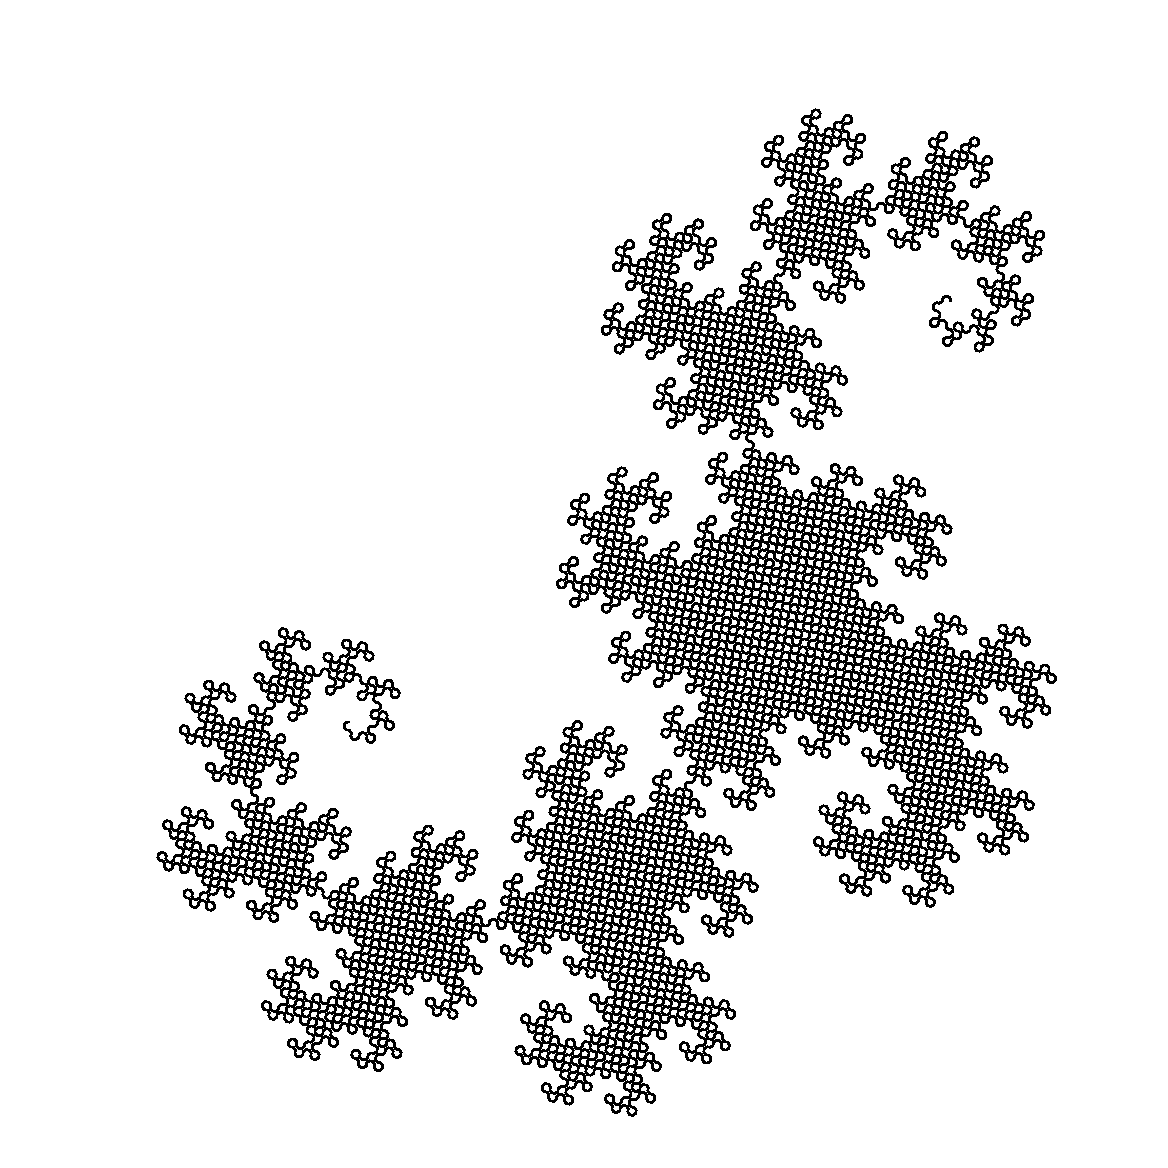
\includegraphics[width=0.9\textwidth]{krunimir/examples/dragon}
  \caption{Příklad obrázku vykresleného pomocí Krunimírova jazyka (Dračí křivka)}
  \label{fig:krunimir-dragon}
\end{figure}

\section{Popis jazyka}

Uživatel má k dispozici několik primitivních kreslících funkcí:

\begin{description}
\item[@t{forward(d)}] Želva se posune vpřed o @t{d} jednotek (pixelů).
Pokud je tloušťka pera kladná, zanechá za sebou čáru vedoucí z původní pozice do
nové. Takovýto pohyb se považuje za jeden \emph{tah}.
\item[@t{right(a)}, @t{left(a)}] Želva se otočí doprava, resp. doleva o
@t{a} stupňů.
\item[@t{pen(s)}] Nastaví tloušťku pera na @t{s}
\item[@t{color(r, g, b)}] Nastaví barvu pera, @t{r}, @t{g} a
@t{b} jsou jednotlivé složky modelu RGB v rozsahu 0 až 255.
\end{description}

Jazyk dále umožňuje použít jednoduchou podmínku a cyklus:

\begin{description}
\item[@t{if(x) \{ ... \}}] Vykoná příkazy v těle podmínky právě když je
@t{x} kladné.
\item[@t{repeat(x) \{ ... \}}] Vykoná příkazy @t{x}-krát, je-li
@t{x} kladné.
\end{description}

Uživatel může definovat vlastní procedury a volat je:

\begin{description}

\item[@t{define 
  \textsl{procedura}(\textsl{p1},\textsl{p2},...)
  \{ ... \}
}]
  Definuje proceduru \textsl{procedura}, která má libovolný počet parametrů
  (\textsl{p1}, \textsl{p2}, ...). Tyto parametry mohou být v těle procedury
  použity ve výrazech a nabývají hodnoty předané v místě volání.

\item[@t{\textsl{procedura}(\textsl{arg1},\textsl{arg2},...)}]
  Zavolá proceduru \textsl{procedura} s argumenty (\textsl{arg1}, \textsl{arg2},
  ...). Procedura musí být definována \emph{před} svým voláním a může být
  rekurzivní.

\end{description}

Poslední a nejzajímavější struktura je rozdvojení:

\begin{description}
\item[@t{split \{ ... \}}] Vytvoří klon aktuální želvy, která vykoná
příkazy v těle struktury @t{split}, přičemž původní želva pokračuje ve vykonávání
dalších příkazů. Všechny želvy se pohybují paralelně, vždy všechny provedou
jeden \emph{krok}, poté druhý atd.
\end{description}

Jako argumenty při volání procedur lze používat výrazy vytvořené z celočíselných
literálů, parametrů aktuální procedury, binárních operátorů @t{+}, @t{-},
@t{*} a @t{/} (celočíselné dělení) a negace pomocí operátoru
@t{-}. Ve výrazech je možno používat závorky @t{(} a @t{)},
priorita a asociativita operátorů je jako v matematice.

\subsection{Příklady}

Uvedeme si několik příkladů, které ilustrují využití veškerých příkazů
Krunimírova jazyka. Výstupy těchto příkladů jsou na obrázku
\ref{fig:krunimir-examples}.

\subsubsection{Čtverec (\ref{fig:krunimir-square1})}

Jednoduchý kód, který vykreslí čtverec. 
\lstinputlisting[style=krunimir]{krunimir/examples/square1.txt}

\subsubsection{Mřížka čtverců (\ref{fig:krunimir-squares})}

V této ukázce využijeme procedury, abychom kód rozdělili na menší a přehlednější
části.
\lstinputlisting[style=krunimir]{krunimir/examples/squares.txt}

\subsubsection{Binární strom (\ref{fig:krunimir-bintree})}

Při vykreslování stromů prokáže svoji užitečnost příkaz @t{split}.
\lstinputlisting[style=krunimir]{krunimir/examples/bintree.txt}

% příklady a jejich výsledky by opravdu neměly utéct někam pryč, proto H
\begin{figure}[H]
  \centering

  \begin{subfigure}{0.3\textwidth}
    \centering
    
\includegraphics[width=\textwidth]{krunimir/examples/square1}
    \caption{Čtverec}\label{fig:krunimir-square1}
  \end{subfigure}
  ~
  \begin{subfigure}{0.3\textwidth}
    \centering
    
\includegraphics[width=\textwidth]{krunimir/examples/squares}
    \caption{Mřížka čtverců}\label{fig:krunimir-squares}
  \end{subfigure}
  ~
  \begin{subfigure}{0.3\textwidth}
    \centering
    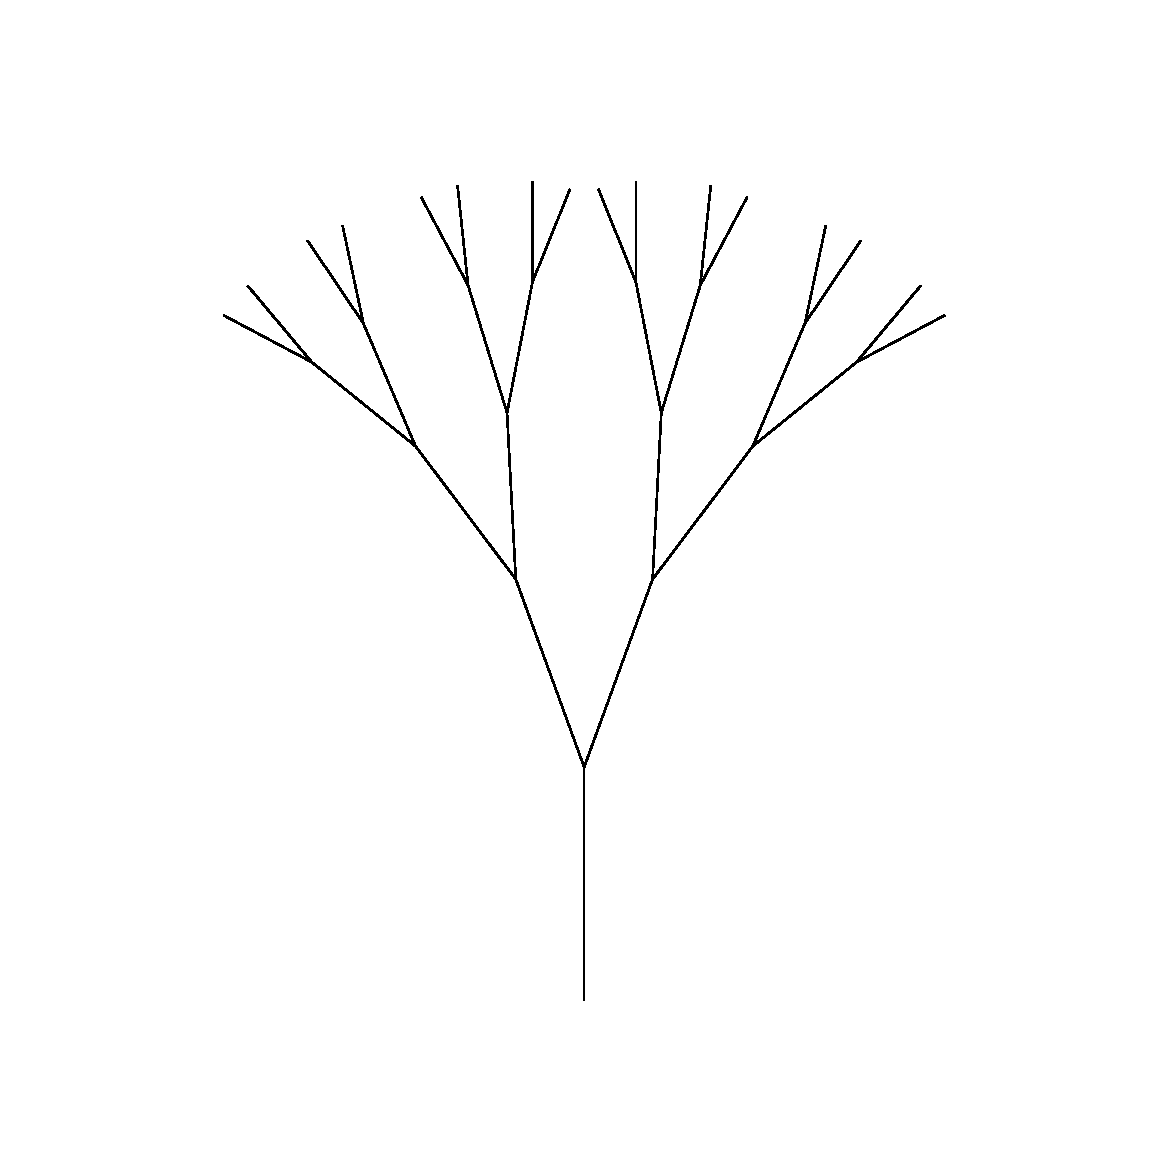
\includegraphics[width=\textwidth]{krunimir/examples/bintree}
    \caption{Binární strom}\label{fig:krunimir-bintree}
  \end{subfigure}

  \caption{Výsledné obrázky z příkladů}
  \label{fig:krunimir-examples}
\end{figure}

\section{Analýza}

Problém si můžeme rozdělit na tři části:

\begin{enumerate}

\item \emph{Syntaktická analýza} (\uv{parsování}) zpracuje vstupní řetězec na
  \emph{abstraktní syntaktický strom}, který zachycuje strukturu programu ve
  formě, která je jednoduše zpracovatelná v dalších fázích.

\item Následuje \emph{vyhodnocení}, kdy ze syntaktického stromu vypočteme
  výslednou stopu (ve vektorové podobě jako seznam úseček).

\item Poslední částí je \emph{vykreslení}, které vykreslí vyhodnocenou stopu do
  obrázku. Budeme exportovat do rastrových obrázků formátu PNG a vektorových
  formátu SVG.

\end{enumerate}

Pomocí tohoto jednoduchého rozdělení můžeme naše řešení rozvrhnout do sedmi
modulů:

\begin{description}

\item @t{Krunimir.Main} exportuje @t{main}, která slouží jako rozhraní s
uživatelem. \footnote{Podobně jako funkce @t{main()} v jazyku C}
  @idx{Krunimir.Main}
  @idx{Krunimir.Main.main}

\item @t{Krunimir.Parser} exportuje funkci @t{parse}, která z textového
zápisu programu vytvoří syntaktický strom (nebo syntaktickou chybu).
  @idx{Krunimir.Parser}
  @idx{Krunimir.Parser.parse}

\item @t{Krunimir.Ast} definuje datové typy, které reprezentují syntaktický
strom.
  @idx{Krunimir.Ast}

\item @t{Krunimir.Evaluator} poskytuje funkci @t{eval}, která ze
syntaktického stromu vypočte výslednou stopu.
  @idx{Krunimir.Evaluator}
  @idx{Krunimir.Evaluator.eval}

\item @t{Krunimir.Trace} definuje datové typy a funkce spojené se stopou želvy.
  @idx{Krunimir.Trace}

\item @t{Krunimir.PngRenderer} exportuje funkci @t{renderPng}, která vykreslí
  stopu jako PNG obrázek.
  @idx{Krunimir.PngRenderer}
  @idx{Krunimir.PngRenderer.renderPng}

\item @t{Krunimir.SvgRenderer} poskytuje funkci @t{renderSvg}, jenž uloží stopu
  ve vektorovém formátu SVG.
  @idx{Krunimir.SvgRenderer}
  @idx{Krunimir.SvgRenderer.renderSvg}

\end{description}

\input{krunimir/Krunimir/Main.lhs}
\input{krunimir/Krunimir/Ast.lhs}
\input{krunimir/Krunimir/Parser.lhs}
\input{krunimir/Krunimir/Trace.lhs}
\input{krunimir/Krunimir/Evaluator.lhs}
\input{krunimir/Krunimir/PngRenderer.lhs}
\input{krunimir/Krunimir/SvgRenderer.lhs}

\section{Příklady}

Závěrem uvedeme několik rozsáhlejších příkladů, kdy využijeme želví grafiku k
vykreslení několika známých fraktálů. 

\subsection{Hilbertova křivka}

\lstinputlisting[style=krunimir]{krunimir/examples/hilbert.txt}

\begin{figure}[p]
  \centering
  
\includegraphics[width=0.9\textwidth]{krunimir/examples/hilbert}
  \caption{Hilbertova křivka}\label{fig:krunimir-hilbert}
\end{figure}

\subsection{Kochova vločka}

\lstinputlisting[style=krunimir]{krunimir/examples/koch.txt}

\begin{figure}[p]
  \centering

  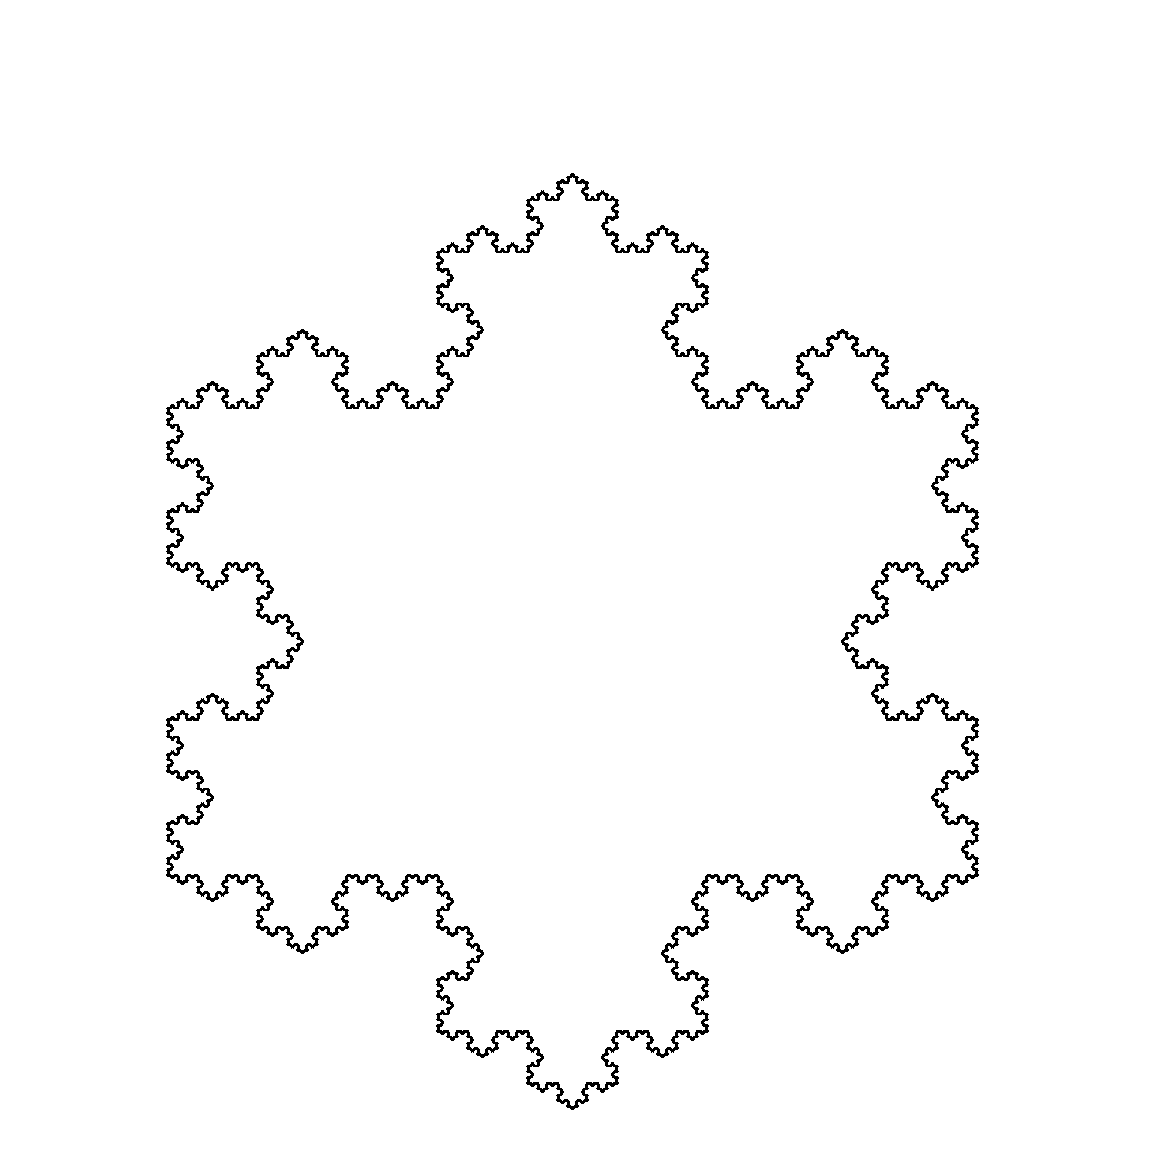
\includegraphics[width=0.9\textwidth]{krunimir/examples/koch}
  \caption{Kochova vločka}\label{fig:krunimir-koch}
\end{figure}

\subsection{Sierpińského křivka}

\lstinputlisting[style=krunimir]{krunimir/examples/sierpinski.txt}

\begin{figure}[p]
  \centering

  
\includegraphics[width=0.9\textwidth]{krunimir/examples/sierpinski}
  \caption{Sierpińského křivka}\label{fig:krunimir-sierpinski}
\end{figure}

\subsection{Gosperova křivka}

\lstinputlisting[style=krunimir]{krunimir/examples/gosper.txt}

\begin{figure}[p]
  \centering

  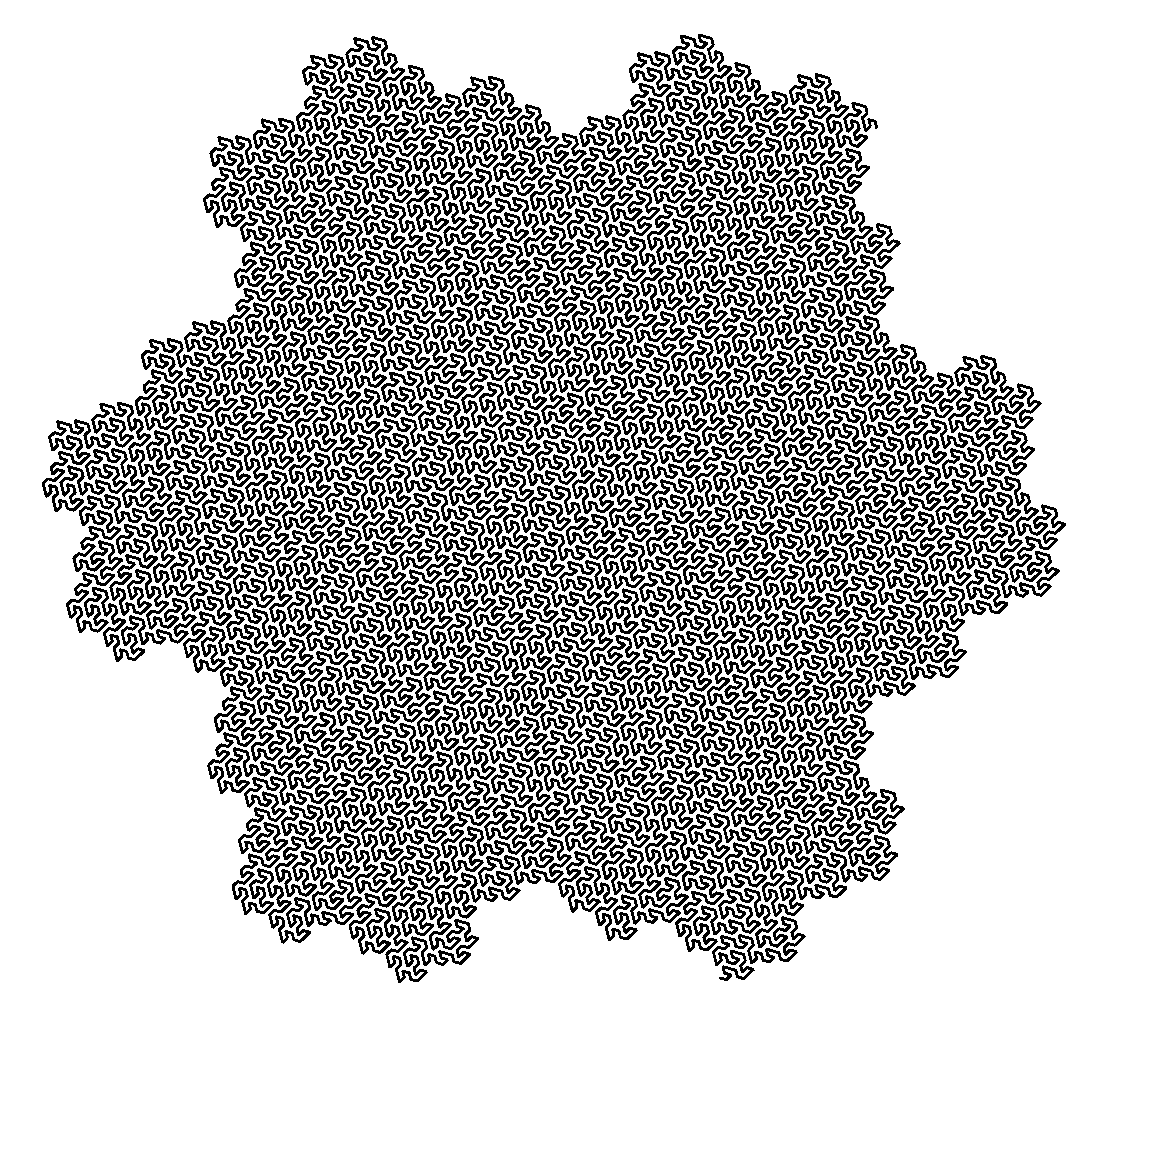
\includegraphics[width=0.9\textwidth]{krunimir/examples/gosper}
  \caption{Gosperova křivka}\label{fig:krunimir-gosper}
\end{figure}

\subsection{Křivka arrowhead}

\lstinputlisting[style=krunimir]{krunimir/examples/arrowhead.txt}

\begin{figure}[p]
  \centering

  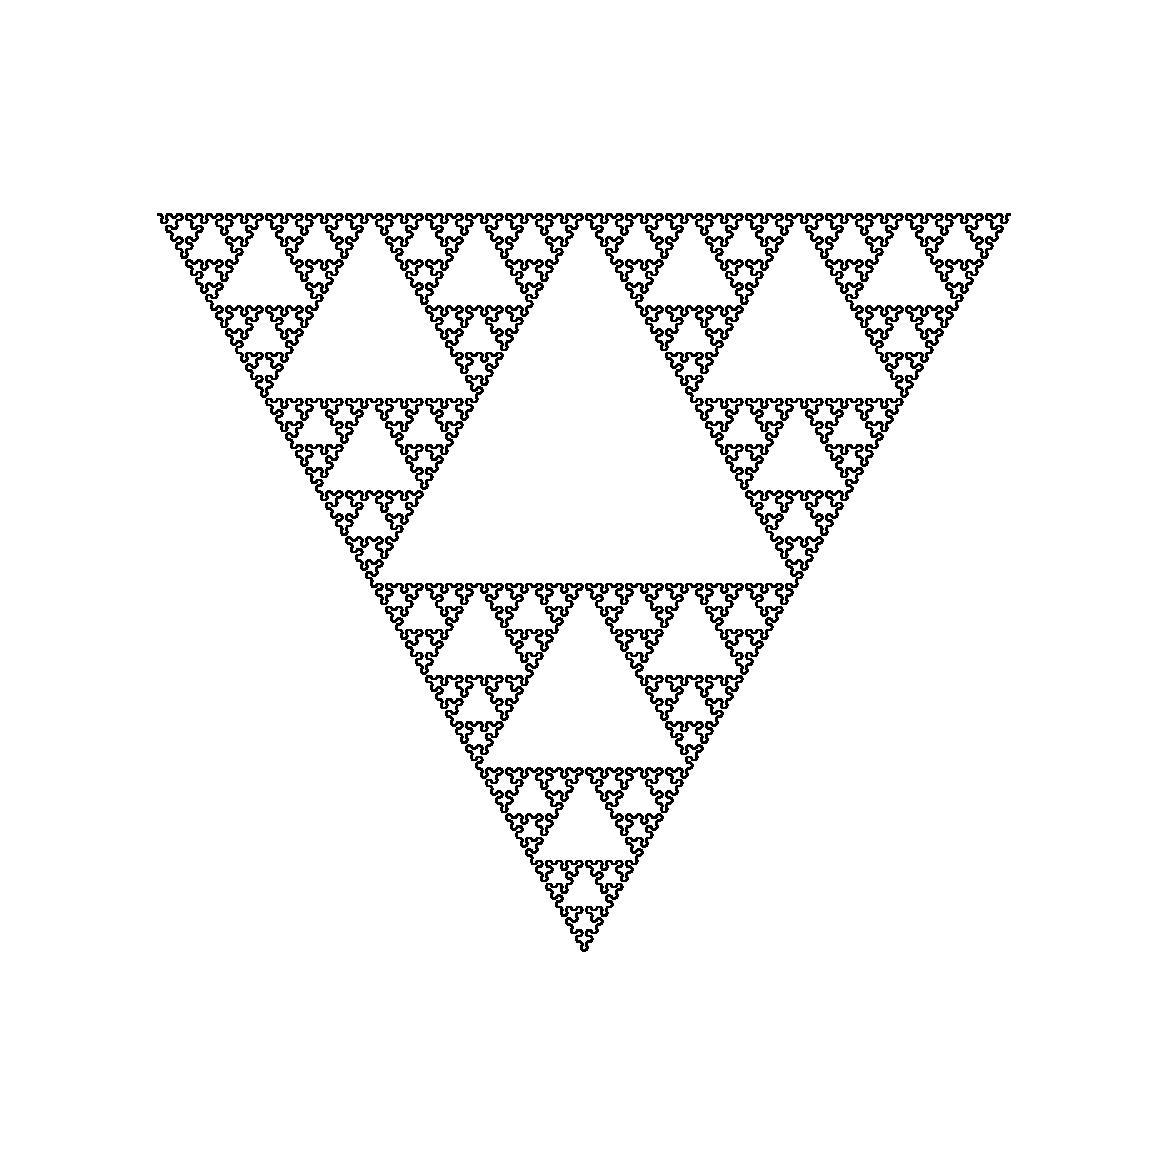
\includegraphics[width=0.9\textwidth]{krunimir/examples/arrowhead}
  \caption{Křivka arrowhead}\label{fig:krunimir-arrowhead}
\end{figure}

